\documentclass{article}
\usepackage{graphicx} % Required for inserting images

\title{Group 5 lab 1 report}
\author{Ashley Björs,Elliot Bodin,Daniel Rytenberg,Jonas Gerne}
\date{January 2024}

\begin{document}
\maketitle

\section{LUT list}


\begin{figure}[h]
    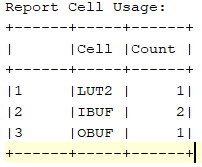
\includegraphics[width=5cm]{{images/lut_step1}}
    \centering
    \caption{This is the LUT list of step 1}
\end{figure}

\begin{figure}[h]
    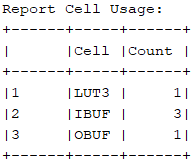
\includegraphics[width=5cm]{{images/lut_step2}}
    \centering
    \caption{This is the LUT list of step 2}
\end{figure}
    
\begin{figure}[h]
    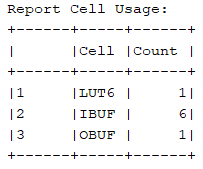
\includegraphics[width=5cm]{{images/lut_step3}}
    \centering
    \caption{This is the LUT list of step 3}
\end{figure}

\begin{figure}[h]
    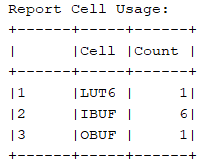
\includegraphics[width=5cm]{{images/lut_step4}}
    \centering
    \caption{This is the LUT list of step 4}
\end{figure}

\begin{figure}[h]
    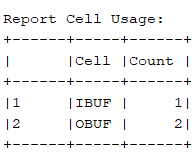
\includegraphics[width=5cm]{{images/lut_step5}}
    \centering
    \caption{This is the LUT list of step 5}
\end{figure}
              
\clearpage

\section{Simulations}


\begin{figure}[h]
    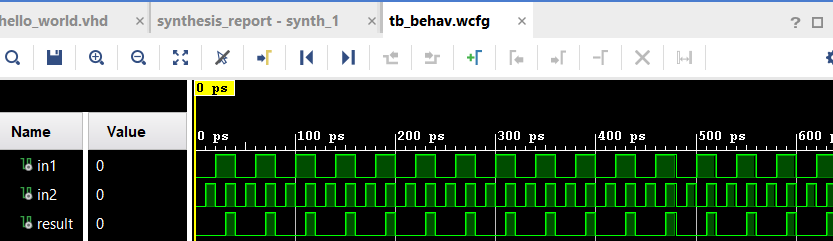
\includegraphics[width=13cm]{{images/sim_step1}}
    \centering
    \caption{This is the simulation of step 1}
\end{figure}

\begin{figure}[h]
    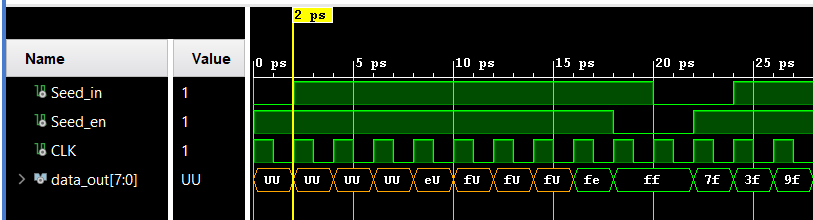
\includegraphics[width=13cm]{{images/sim_step2}}
    \centering
    \caption{This is the simulation of step 2}
\end{figure}

The following components are 3 diffrent ways to implement an 4 to one bit mutex. 
The IO are the following:

\begin{itemize}
    \item i0-i3 are inputs.
    \item s0,s1 are select for the following input values.
    \item out0 are the output from the 4 to 1 mutex.
  \end{itemize}

\begin{figure}[h]
    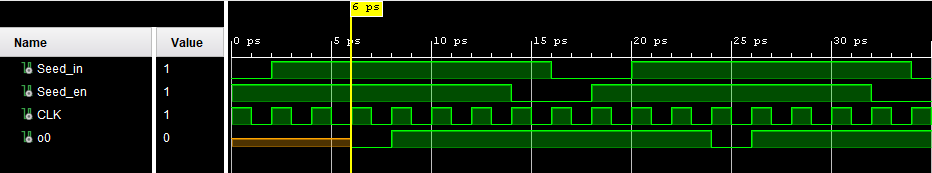
\includegraphics[width=13cm]{{images/sim_step3}}
    \centering
    \caption{This is the simulation of step 3}
\end{figure}

\begin{figure}[h]
    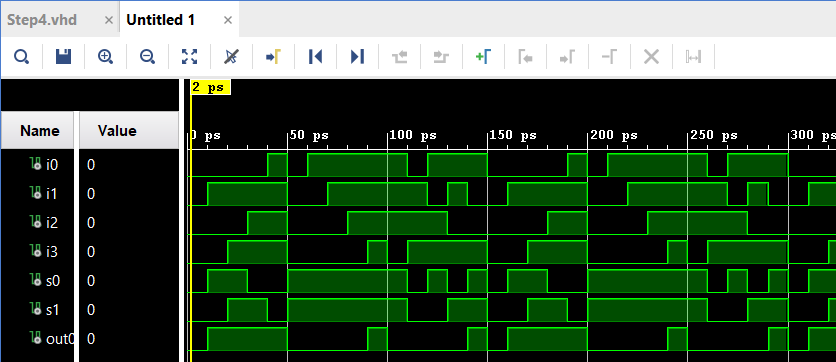
\includegraphics[width=13cm]{{images/sim_step4}}
    \centering
    \caption{This is the simulation of step 4}
\end{figure}

\begin{figure}[h]
    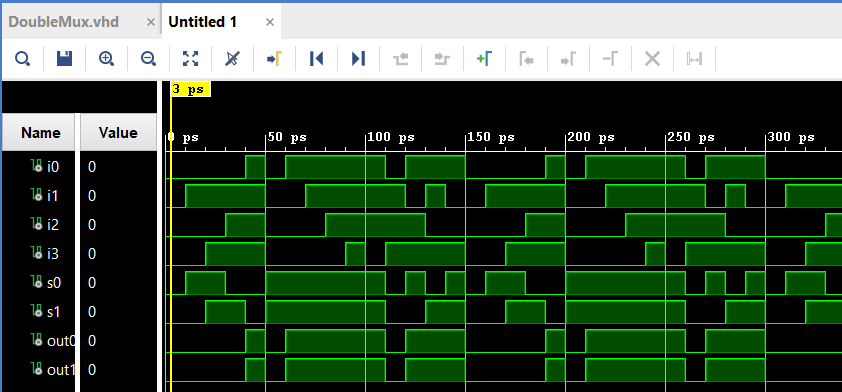
\includegraphics[width=13cm]{{images/sim_step5}}
    \centering
    \caption{This is the simulation of step 5}
\end{figure}
\end{document}
